\documentclass[a4paper,12pt]{report}
\usepackage[utf8]{inputenc}
\usepackage{graphicx} % Para incluir imágenes
\usepackage{tocloft} % Para personalizar índices
\usepackage{hyperref} % Para enlaces
\usepackage{titlesec} % Para personalizar títulos
\usepackage[backend=biber,style=ieee]{biblatex} % Bibliografía con biblatex
\usepackage{subcaption} % Para el collage de imagenes

\usepackage{indentfirst} % Para la sangria

\usepackage{ragged2e}

\usepackage{amsmath} % Pack Nomenclatura Matemática
\usepackage{amsmath, amssymb}
\usepackage{bm}


% INDICE ------------------------------------------------------

% Cambiar título del índice
\renewcommand{\contentsname}{Índice General}

% Personalizar el formato de capítulos en el índice
\renewcommand{\cftchapleader}{\cftdotfill{\cftdotsep}} % Puntos entre títulos y números
\renewcommand{\cftchapdotsep}{1.5} % Ajusta la separación entre puntos

% CAPITULOS ---------------------------------------------------

% Redefinir el formato del capítulo y eliminar el espacio superior
\titleformat{\chapter}[block]
    {\normalfont\LARGE\bfseries\centering} % Estilo: tamaño grande, negrita, centrado
    {} % Sin prefijo como "Chapter"
    {0pt} % Sin espacio entre el prefijo y el título
    {\LARGE} % Estilo del título del capítulo
\titlespacing*{\chapter}{0pt}{-50pt}{20pt} % Ajustar espaciado: elimina espacio superior

% BIBLIOGRAFÍA -----------------------------------------------------

% Carga el archivo .bib
\addbibresource{bibliografia.bib} % Archivo con las referencias

% SANGRÍA -----------------------------------------------------
\setlength{\parindent}{15pt} % Añade la sagría como tal
\setlength{\parskip}{10pt} % Añade espacio entre párrafos
% -------------------------------------------------------------
\begin{document}
\justifying
% Portada
\begin{titlepage}
    \thispagestyle{empty} % Sin numeración ni encabezado
    \begin{center}
    \centering
    \vspace*{-3cm} % Espaciado superior
    \includegraphics[width=1\textwidth]{images/logo-uax.png} % Logo opcional
    \vspace{1cm}

    {\Large \textbf{UNIVERSIDAD ALFONSO X EL SABIO}} \\[0.5cm] % Título principal
    {\large \textbf{FACULTAD BUSINESS AND TECH}} \\[1cm] % Título principal

    {\LARGE \textbf{Estudio de los fenotipos conductuales, la persistencia y la cooperación en redes sociales artificiales a través de teoría de juegos} } \\[1cm] % Subtítulo opcional

    {\large \textbf{Miguel González González}} \\[3 cm]

    {\Large \textbf{TRABAJO DE FIN DE GRADO}} \\[0.5cm]
    {\Large \textbf{GRADO EN INGENIERÍA MATEMÁTICA}}
    

    \vfill % Para alinear el texto al final de la página
    \textbf{Villanueva de la Cañada, 2025} \\

    \vspace*{1cm}
    \end{center}
\end{titlepage}
\newpage

\begin{titlepage}
    \thispagestyle{empty}
    \begin{center}
        \vspace*{-2.5cm}
        \includegraphics[width=0.18\textwidth]{images/logo_blanco_y_negro.png}

        \vspace{1cm}
        {\bfseries\LARGE UNIVERSIDAD ALFONSO X EL SABIO}

        \vspace{1.5cm}
        {\large Grado en Ingeniería Matemática}

        \vspace{2.5cm}
        {\bfseries\Large
        Estudio de los fenotipos conductuales,\\
        la persistencia y la cooperación en redes\\
        sociales artificiales a través de teoría de juegos}
    \end{center}    
    \vspace{2.5cm}
    {\large \textbf{ALUMNO:} Miguel González González} \\[0.5cm]
    {\large \textbf{NP:} 138683} \\[0.5cm]
    {\large \textbf{TUTOR DEL TRABAJO:} Hugo Andrea Galindo Beleña} \\[0.5cm]        
    {\large \textbf{FECHA DE PRESENTACIÓN:} XX/07/2025} \\[2cm]        
    \textbf{Firma del director:}
    \hfill
    \textbf{Firma del alumno:}
\end{titlepage}


% Índices
\newpage
\tableofcontents % Índice general

\newpage

% ------------------------------------------------------------

% Introducción
\chapter{Introducción}

Los seres humanos, como seres sociales y racionales, se ven involucrados de manera involuntaria en interacciones sociales en las que los implicados actúan de manera estratégica. Del mismo modo, los individuos implicados anticipan las posibles respuestas de los demás actores, buscando el resultado que más les favorece.

Algunas de estas interacciones sociales incluyen dilemas, donde el interés propio y el colectivo se ven enfrentados, conflicto entre la racionalidad individual y colectiva, entre intereses propios a corto plazo e intereses colectivos a largo plazo \cite{dawes1980social,kollock1998social,vanLange2013psychology}. Estos y otros escenarios han sido estudiados en economía, psicología y sociología, utilizando un marco teórico para comprender como los actores acometen cooperación o conflicto.

La Teoría de Juegos tradicional se basa en que los actores son racionales y egoistas en su totalidad, pero sabemos que las personas no siempre son totalmente racionales, es decir, que no siempre se persiguen objetivos meramente egoistas.
Es así como se introduce la nueva Teoría de Juegos conocida como Teoría de Juegos Conductual\cite{camerer2003behavioral,kagel1995handbook},y posteriormente la Evolutiva\cite{sigmund2010calculus,gintis2009game}, que ya no solamente trata a los tomadores de decisiones como racionales egoistas, sino que incorporan factores psicológicos, racionalidad imperfecta, capacidad de aprendizaje y experiencias, además de ser capaces de cooperar cuando la teoría predice lo contrario.

Estos y otros trabajos han respaldado que la racionalidad no es suficiente para predecir el comportamiento humano, ya que la cooperación puede surgir sin necesidad de un plan centralizado. La cooperación también depende de la situacion de los decisores, importando mucho la información de la que disponen, el contexto de las decisiones y las estrategias de cada uno \cite{sigmund2010calculus,gintis2009game,myerson1991game}.

En este contexto, resulta interesante analizar cómo distintas disposiciones estratégicas conviven y evolucionan dentro de una población. En vez de dar por sentado que todos los individuos actuan de manera homogenea, varios estudios han identificado la existencia de fenotipos conductuales consistentes, que guian las decisiones en dilemas sociales \cite{paper_principal}. Añadir tal diversidad estratégica permite una aproximación más realista a los modelos de comportamiento, buscando nuevas formas de entender fenómeos como la aparición espontanea de cooperación o la resistencia al cambio.

\newpage

Este trabajo de fin de grado propone un modelo basado en la teoría de juegos evolutiva, en el que una población de agentes heterogéneos  interactúa de manera local sobre una retícula periódica. Cada jugador sigue un comportamiento estratégico asociado a su fenotipo, además de un nivel de persistencia que condiciona su capacidad de adaptación. A través de simulaciones, se estudia cómo el contexto loca y global,y los parámetros que regulan el cambio influyen en la dinámica colectiva del sistema.

El objetivo principal es qué configuraciones favorecen a la cooperación sostenida en el tiempo, variando las distribuciones de los fentoipos, identificar qué fenotipos tienden a prevalecer bajo distintas condiciones y analizar que tan estable es el sistema ante perturbaciones. Este trabajo no solamente trata de replicar el comportamiento observado de manera empírica, sino también trata de ofrecer un marco flexible para comprender mejor la complejidad ligada a los procesos de decisión social.

% ------------------------------------------------------------
% Revisión de la literatura
\chapter{Revisión de la literatura}

Dentro del campo de la Teoría de Juegos, hay muchos estudios que hablan sobre las decisiones irracionales que toman ciertos individuos en situaciones estratégicas colectivas, incluso cuando la respuesta óptima para el individuo era clara. Esto se debe a que no todos los seres humanos somos racionales y egoístas en su totalidad, y dependemos de otros factores como la moralidad, la confianza o el conocimiento para tomar decisiones \cite{dawes1980social}. Hay veces que estas malas decisiones se deben a un nivel cognitivo bajo, pero en otras ocasiones, se trata de un dilema mayor o dilema social, en el cual las decisiones contraponen el bien individual y el colectivo \cite{kollock1998social}.

Los dilemas sociales han sido estudiados en muchos contextos diferentes y con muchas variantes, para poder entender qué factores influyen en las negociaciones y en qué circunstancias se da la cooperación. La cooperación no depende solamente de la racionalidad, hay muchas otras variables que complican el estudio de la posible cooperación entre dos individuos, como por ejemplo: reciprocidad, equidad, contexto, obligaciones morales, conocimientos, razonamientos estratégicos, experiencias pasadas, entre muchas otras \cite{sigmund2010calculus,camerer2003behavioral,kagel1995handbook,gintis2009game}.

El punto es, que hay individuos que aún dándoles razones suficientes para no cooperar, cooperan contra sus propios beneficios. Pareciera que el hecho de cooperar o no en estos dilemas sociales fuera más allá de todas las variables previamente mencionadas, como si fuera algo intrínseco de cada individuo.

Existe un estudio que avala este punto de vista, dando la conclusión de la existencia de cuatro fenotipos conductuales en los juegos diádicos como el del dilema del prisionero. Estos cuatro fenotipos fueron definidos de la siguiente manera:

\begin{itemize}
\item \textbf{Envidioso:} Quiere obtener mejor resultado que su oponente, sin importar si ello implica una menor ganancia total.
\item \textbf{Optimista:} Pretende buscar el mejor resultado mutuo posible, incluso si esto perjudica a su ganancia individual.
\item \textbf{Pesimista:} Evita el peor resultado, eligiendo siempre lo más seguro y suponiendo el peor escenario como el más probable.
\item \textbf{Confiado:} Siempre busca la cooperación y espera lo mismo de su oponente.
\end{itemize}

También existe un quinto fenotipo, conocido como indefinido, que representa a aquellos individuos cuyo comportamiento no sigue a una estrategia clara o coherente. Este tipo de jugador actúa de forma aleatoria, lo que introduce un elemento de incertidumbre en las dinámicas del juego. Aunque minoritario, su presencia puede alterar la evolución del sistema y a su vez la dinámica de cooperación que debería seguir \cite{paper_principal}.

Este artículo nos puede llevar a la conclusión de que, en escenarios estratégicos con dilemas sociales, se puede predecir el comportamiento humano. La identificación de fenotipos estratégicos recurrentes sugiere que es posible anticipar, al menos de manera parcial, las decisiones de los individuos en contextos de interacción estratégica. Esto abre la puerta a modelos conductuales más ajustados a la realidad, que incorporan la diversidad de perfiles y la influencia del entorno.

Existe otro estudio que habla de la persistencia de las estrategias que siguen los individuos en entornos locales frente a globales, donde los actores adaptan su nivel de persistencia comparando la situación local frente a la global \cite{liming2022adaptative}. Los individuos mantendrán o cambiarán su estrategia en función de si su rendimiento local es mejor que el rendimiento medio global.

Esta práctica lleva a mejorar los niveles de persistencia entre los cooperadores promoviendo la cooperación en juegos evolutivos, cosa que de no ser por estas comparativas de entornos sería complicado de mantener porque los agentes egoístas tienen más incentivos para actuar de una manera oportunista.

Hay veces, que en estos juegos diádicos la cooperación no es la mejor estrategia, y en otras situaciones como en las sociedades humanas, la cooperación y coordinación entre los actores promueven el surgimiento y mantenimiento de las sociedades, poniendo como ejemplo a Japón. Existen conceptos que fomentan estas prácticas, como la de la "reciprocidad institucionalizada" que implica incorporar la estrategia recíproca como institución formal para facilitar la cooperación y reducir la probabilidad de comportamientos oportunistas \cite{Ozono2016Reciprocity}.

Como sociedad, es importante colaborar y cooperar para promover y mantener la comunidad, pero dentro de las comunidades existe más de un tipo de fenotipo, no solamente los colaboradores y los oportunistas, siendo un dilema la siguiente cuestión: ¿Hasta que punto afecta que una comunidad sea más o menos colaborativa? ¿Se desarrollará de una mejor forma una comunidad con una mayoría de un fenotipo mejor que otra? ¿Qué tipos de fenotipos son capaces de convivir mejor dentro de una comunidad y cuáles en cambio provocarán que su entoro tenga un peor rendimiento? 

% ------------------------------------------------------------
% Formulación matemática / Modelo
\chapter{Formulación matemática}

Para el modelo matemático, vamos a simular una población a través de una combinación entre el método de Monte Carlo y una retícula periódica.
La Simulación de Monte Carlo es una técnica matemática que usa números aleatorios y probabilidad para entender el impacto del riesgo de un modelo en la realidad.
En este caso, el modelo será una población dividida en vecindarios o vecinos los cuales solo interactuarán entre ellos, mezclando fenotipos en unos vecindarios y dejando vecindarios de otros fenotipos de mayoritariamente.
Las interacciones se basan en juegos de la Teoría de Juegos estáticos con pesos aleatorios.
Con este modelo trataremos de entender cómo las perturbaciones aleatorias se propagan al resto del modelo.

\section{Marco del Modelo Matemático}

Consideramos una población de individuos dispuestos sobre una retícula de tamaño \( L \times L\), con condiciones de periodicidad en los bordes. Cada nodo representa un único jugador que interactua solamente con sus vecinos adyacentes.
A cada jugador \( i \) se le asigna una estrategia fenotípica o fenotipo estratégico la cual puede evolucionar durante la simulación. Los fenotipos que existen en la simulación son:

\[
\Psi = \{ \text{Envidioso (E)}, \text{Optimista (O)}, \text{Pesimista (P)}, \text{Altruista (A)}, \text{Aleatorio (R)} \}
\]

Cada interacción entre individuos se modela como un juego \( 2 \times 2 \), con la siguiente matriz de pagos:

\[
\begin{array}{c|cc}
  & C & D \\
\hline
C & 1 & S \\
D & T & 0 \\
\end{array}
\quad \text{donde } 0 \leq T \leq 2, \quad -1 \leq S \leq 1
\]

Los jugadores eligen entre cooperar (C) o traicionar (D), siguiendo una de las siguientes reglas fenotípicas:

\newpage


\begin{figure}[h!]
    \centering
    \includegraphics[width=1\textwidth]{images/fenotipos_modelo_teorico.png}
    \label{fig:fenotipos-modelo}
    \caption{Modelo teórico de los fenotipos}
\end{figure}

Cada jugador adopta una estrategia en función del contexto del juego en el que se encuentra. Denotamos por \( s \in  S \)  al estado del juego o situación estratégica percibida por el jugador, la cual incluye la información relevante para su toma de decisiones. En nuestro caso, este estado está determinado por los valores de los parámetros de la matriz de pagos: la tentación \( T \), el castigo \( 0 \), la recompensa mutua \( 1 \), y el valor de \( S \), que representa la ganancia al cooperar frente a un oponente traidor. Así, cada fenotipo puede ser descrito como una función de decisión
\[
\psi : S \rightarrow \{C, D\}
\]
donde \( \psi(s) \) devuelve la estrategia elegida (cooperar \( C \) o traicionar \( D \)) según el tipo de jugador y el estado \( s \) percibido.


\begin{itemize}
  \item \textbf{Envidioso (E):} Coopera solo si recibe un pago mayor que el del oponente:
  \[
  E(s) =
  \begin{cases}
    C & \text{si } S > T \\
    D & \text{si } S \leq T
  \end{cases}
  \]

  \item \textbf{Optimista (O):} Busca maximizar su beneficio:
  \[
  O(s) =
  \begin{cases}
    C & \text{si } T < 1 \\
    D & \text{si } T > 1
  \end{cases}
  \]

  \item \textbf{Pesimista (P):} Minimiza el riesgo, esperando el peor escenario:
  \[
  P(s) =
  \begin{cases}
    C & \text{si } S > 0 \\
    D & \text{si } S \leq 0
  \end{cases}
  \]

  \item \textbf{Altruista (A):} Coopera incondicionalmente:
  \[
  A(s) = C
  \]

  \item \textbf{Aleatorio (R):} Coopera o traiciona con igual probabilidad:
  \[
  R(s) =
  \begin{cases}
    C & \text{con probabilidad } \frac{1}{2} \\
    D & \text{con probabilidad } \frac{1}{2}
  \end{cases}
  \]
\end{itemize}
\justifying
A cada fenotipo \( \psi_i \in \Psi \) se le asocia una regla de comportamiento \( \mathcal{R}_{\psi^\alpha} \), que determina la probabilidad estratégica o la elección estratégica del jugador en función del contexto del juego y del entorno.

Podemos representar la probabilidad de cooperación de un jugador con fenotipo \( \psi^\alpha \) en el tiempo \( t \) como:

\[
P_i(t) = \mathbb{P}(s_i(t) = C \mid \psi_i = \psi^\alpha, \mathcal{G}_i(t))
\]

donde \( \mathcal{G}_i(t) \) representa el estado del juego percibido por el jugador \( i \).

Al inicio del modelo, cada jugador es asignado a un fenotipo de acuerdo a una distribución de probabilidad con:

\[
\mathbb{P}(\psi_i = \psi^\alpha) = \pi_\alpha, \quad \sum_{\alpha=1}^{M} \pi_\alpha = 1
\]

Las probabilidades de cada fenotipo vienen determinadas por "Humans display a reduced set of consistent behavioral phenotypes in dyadic games "\cite{paper_principal}. Estas probabilidades son:

\begin{center}
\small
\begin{tabular}{l}
\textbf{Envidioso}: 30\% \\
\textbf{Pesimista}: 21\% \\
\textbf{Optimista}: 20\% \\
\textbf{Confiado}: 17\% \\
\textbf{Indefinido}: 12\% \\
\end{tabular}
\end{center}

Cada jugador posee un nivel de persistencia el cual puede variar con el tiempo \(t\), denotado por \( \tau_i(t) \in [\tau_D, \tau_U] \). Además se introduce un contador \( \theta_i \), que registra cuántos pasos lleva el jugador manteniendo su estrategia actual.

Definimos el entorno local del jugador \( i \) como una función \( \phi_i(t) \) que depende de los fenotipos de sus vecinos:

\[
\phi_i(t) = \frac{1}{k_i} \sum_{j \in \mathcal{N}_i} f(s_j(t))
\]

donde \( \mathcal{N}_i \) es el conjunto de vecinos inmediatos de \( i \), \( k_i = |\mathcal{N}_i| \), y \( f(\cdot) \) es una función que mapea el fenotipo a una medida cuantificable de cooperación.

Asimismo, se define el entorno global \( \phi(t) \) como:

\[
\phi(t) = \frac{1}{N} \sum_{j=1}^{N} f(s_j(t))
\]

Cada jugador compara su entorno local con el global. Si \( \phi_i(t) > \phi(t) \), se considera que se encuentra en un entorno favorable y tenderá a aumentar su nivel de persistencia. De lo contrario, lo disminuirá. Esta dinámica se implementa mediante una función tipo Fermi:

\[
P_{\text{incremento}} = \frac{1}{1 + \exp\left( -\frac{ \phi_i(t) - \phi(t) }{K_1} \right)}
\]

donde \( K_1 \) es un parámetro de ruido que controla la sensibilidad a las diferencias de entorno.

Para modelar estos cambios de forma gradual, se introduce el parámetro \( \Delta\tau > 0 \), que controla el incremento o decremento del nivel de persistencia. Así, si el entorno es favorable ,es decir, el jugador decide aumentar su persistencia, el valor se actualiza como:

\[
\tau_i(t+1) = \min(\tau_i(t) + \Delta\tau, \tau_U)
\]

Y si el entorno es desfavorable, la actualización es:

\[
\tau_i(t+1) = \max(\tau_i(t) - \Delta\tau, \tau_D)
\]

Este mecanismo permite que los jugadores ajusten de forma progresiva su resistencia al cambio de estrategia, dependiendo de la calidad relativa de su entorno local.

Los jugadores solo consideran cambiar su estrategia cuando su temporizador alcanza su nivel de persistencia actual: \( \theta_i \geq \tau_i(t) \). En ese momento, el jugador \( i \) selecciona un vecino \( j \) al azar y considera adoptar su fenotipo con una probabilidad dada por:

\[
W_{s_i \leftarrow s_j}(t) = \frac{1}{1 + \exp\left( -\frac{ \pi_j(t) - \pi_i(t) }{K_2} \right)}
\]

donde \( \pi_i(t) \) y \( \pi_j(t) \) son los pagos acumulados de \( i \) y \( j \), respectivamente, calculados a partir de sus interacciones con sus vecinos, y \( K_2 \) es otro parámetro de ruido.

Una vez imitada la estrategia, el temporizador del jugador se reinicia: \( \theta_i = 0 \). Este mecanismo representa que el individuo ha adoptado un nuevo fenotipo y, por tanto, necesita un nuevo periodo de observación antes de poder plantearse otro cambio. En caso de que no imite al vecino seleccionado, su temporizador aumenta en una unidad, acumulando pasos hasta alcanzar nuevamente su nivel de persistencia \( \tau_i \). Esta dinámica garantiza que los jugadores no cambien de estrategia de manera impulsiva, introduciendo una memoria temporal que modula la frecuencia de los cambios.


% Resultados y discusión
\chapter{Resultados y discusión}

Basandonos en el modelo matemático propuesto en el apartado anterior, crearmos un programa que sigue la simulación de Monte Carlo como es propuesta en el marco teórico \cite{TFG_SimulacionAgentesFenotipos}.
Una vez probado el modelo lo utilizamos para hacer diversas simulaciones, alterando los parámetros y observando qué patrones o ciclos encontramos dados unos parámetros concretos.
Tratamos de entender el funcionamiento de los fenotipos en diferentes entornos, ya sean vecindarios predeterminados como distribuciones o parámetros de ruido varios.
Salvo en simulaciones concretas, la distribución de la retícula será aleatoria, es decir, que las reticulas distribuirán siguiendo las probabilidades establecidas las posiciones de los fenotipos de manera aleatoria. Esto es importante ya que independientemente de que una simulación con ciertos valores para los diferentes parámetros nos de un resultado similar puede suceder que tengamos una distribución que favorezca la progresión de algún fenotipo que no debería progresar.

\vspace{1.5em}
\noindent\textbf{Probabilidades basadas en el marco teórico}
\vspace{0.5em}


Las primeras simulaciones fueron enfocadas a las probabilidades sacadas del arítculo ”Humans
display a reduced set of consistent behavioral phenotypes in dyadic games
” \cite{paper_principal}.

Para las distribuciones del paper con los parámetros \( K_1 = 0.1\) y \( K_2 = 0.1\) obtenemos los siguientes resultados

% Collage de simulación
%TOP
\begin{figure}[h]
    \centering
    \begin{minipage}{0.49\textwidth}
    \centering
    \includegraphics[width=1\textwidth]{images/prob_normal/SIM1/fenotipos_evolucion.png}
    \label{fig:enter-label}
    \end{minipage}
    \hfill
    \begin{minipage}{0.49\textwidth}
    \centering
    \includegraphics[width=1\textwidth]{images/prob_normal/SIM1/cooperacion_global.png}
    \label{fig:enter-label}
    \end{minipage}
\end{figure}
%UNDER
\begin{figure}[h]
    \centering
    \begin{subfigure}[t]{0.49\textwidth}
        \centering
        \includegraphics[width=1\textwidth]{images/prob_normal/SIM2/fenotipos_evolucion.png}
        \label{fig:enter-label}
    \end{subfigure}
    \hfill
    \begin{subfigure}[t]{0.49\textwidth}
        \centering
        \includegraphics[width=1\textwidth]{images/prob_normal/SIM2/cooperacion_global.png}
        \label{fig:enter-label}
    \end{subfigure}
\end{figure}

También realizamos simulaciones cambiando los valores de los parametros \( K_1\) y \( K_2\) para ver que evoluciones tiene la reticula cambiandolos.
Comenzando con cambios realizados dentro de los valores de \( K_1\), donde iremos de menos a más progresivamente.

\newpage

\subsection{Simlaciones variando el parámetro \( K_1 \)}

Para las simulaciones del parámetro \( K_1 \), los valores de el parámetro \( K_2 \) serán siempre 0.1 durante este apartado.

\vspace{1.5em}
\noindent\textbf{Parámetro \( K_1 \) con valor 0.01}
\vspace{0.5em}


Para el parámetro \( K_1 \) con el valor 0.01, las simulaciones a partir de 100 pasos son más inestables. La cooperación global puede caer  o ascender de manera drástica en función de la distribución que siga la retícula.

\begin{figure}[h!]
    \centering
    \begin{minipage}{0.49\textwidth}
    \centering
    \includegraphics[width=1\textwidth]{images/K1/001/fenotipos_evolucion.png}
    \label{fig:enter-label}
    \end{minipage}
    \hfill
    \begin{minipage}{0.49\textwidth}
    \centering
    \includegraphics[width=1\textwidth]{images/K1/001/cooperacion_global.png}
    \label{fig:enter-label}
    \end{minipage}
    \caption{Cooperación global con distribución al 20\%}
\end{figure}

Si reducimos el porcentaje de Optimistas y Altruistas, los Envidiosos y Pesimistas tomarán el control de laretícula y la cooperación global caerá en consecuencia. Por contrapartida, si aumentamos el porcentaje de Oprimistas y Altruistas, y disminuimos el porcentaje de Envidiosos y Pesimistas, la cooperación global aumentará, tomando el control de la retícula los Optimistas y Altruistas.

%TOP
\begin{figure}[h]
    \centering
    \begin{minipage}{0.49\textwidth}
    \centering
    \includegraphics[width=1\textwidth]{images/K1/001/EP/fenotipos_evolucion.png}
    \label{fig:enter-label}
    \end{minipage}
    \hfill
    \begin{minipage}{0.49\textwidth}
    \centering
    \includegraphics[width=1\textwidth]{images/K1/001/EP/cooperacion_global.png}
    \label{fig:enter-label}
    \end{minipage}
    \caption{Mayoría de Envidiosos y Pesimistas}
\end{figure}
%UNDER
\begin{figure}[h]
    \centering
    \begin{subfigure}[t]{0.49\textwidth}
        \centering
        \includegraphics[width=1\textwidth]{images/K1/001/OA/fenotipos_evolucion.png}
        \label{fig:enter-label}
    \end{subfigure}
    \hfill
    \begin{subfigure}[t]{0.49\textwidth}
        \centering
        \includegraphics[width=1\textwidth]{images/K1/001/OA/cooperacion_global.png}
        \label{fig:enter-label}
    \end{subfigure}
    \caption{Mayoría de Optimistas y Altruistas}
\end{figure}

\newpage

\vspace{1.5em}
\noindent\textbf{Parámetro \( K_1 \) con valor 0.3}
\vspace{0.5em}


Para el parámetro \( K_1 \) con el valor 0.01, manteniendo como distribución un 20\% para cada fenotipo, en la mayoría de las simulaciones dominan la retícula los fenotipos cooperadores.
Disminuyendo la probabilidad de aparición de estos fenotipos en la retícula también hay casos en los que destacan, pero mayoritariamente dominan la reticula los fenotipos no cooperadores.

%TOP
\begin{figure}[h]
    \centering
    \begin{minipage}{0.49\textwidth}
    \centering
    \includegraphics[width=1\textwidth]{images/K1/030/EP/fenotipos_evolucion.png}
    \label{fig:enter-label}
    \end{minipage}
    \hfill
    \begin{minipage}{0.49\textwidth}
    \centering
    \includegraphics[width=1\textwidth]{images/K1/030/EP/cooperacion_global.png}
    \label{fig:enter-label}
    \end{minipage}
    \caption{Mayoría de Envidiosos y Pesimistas}
\end{figure}
%UNDER
\begin{figure}[h]
    \centering
    \begin{subfigure}[t]{0.49\textwidth}
        \centering
        \includegraphics[width=1\textwidth]{images/K1/030/OA/fenotipos_evolucion.png}
        \label{fig:enter-label}
    \end{subfigure}
    \hfill
    \begin{subfigure}[t]{0.49\textwidth}
        \centering
        \includegraphics[width=1\textwidth]{images/K1/030/OA/cooperacion_global.png}
        \label{fig:enter-label}
    \end{subfigure}
    \caption{Mayoría de Optimistas y Altruistas}
\end{figure}

Es importante saber que en casos en los que la distribución es igualitaria para todos los fenotipos, los favorecidos son los cooperantes.

\newpage

\vspace{1.5em}
\noindent\textbf{Parámetro \( K_1 \) con valor 0.7}
\vspace{0.5em}

En estas simulaciones, se ven favorecidos los fenotipos que durante los primeros pasos se convierten en mayoría de la retícula, y los fenotipos que son minoritarios tienden a desaparecer de la reticula con el a los 120 pasos de la simulación.
Un punto a destacar es que solamente los fenotipos cooperadores tienen la capacidad de remontar  en número dentro de la reticula, es decir, que si empiezan las primeras iteraciones siendo minoría, son los únicos capaces de aumentar en número cuando va evolucionando la retícula.
Mayoritariamente consiguen encontrarse casos en los que destacan los fenotipos cooperadores al final de la simulación.


%TOP
\begin{figure}[h]
    \centering
    \begin{minipage}{0.49\textwidth}
    \centering
    \includegraphics[width=1\textwidth]{images/K1/070/EP/fenotipos_evolucion.png}
    \label{fig:enter-label}
    \end{minipage}
    \hfill
    \begin{minipage}{0.49\textwidth}
    \centering
    \includegraphics[width=1\textwidth]{images/K1/070/EP/cooperacion_global.png}
    \label{fig:enter-label}
    \end{minipage}
    \caption{Mayoría de Envidiosos y Pesimistas}
\end{figure}
%UNDER
\begin{figure}[h]
    \centering
    \begin{subfigure}[t]{0.49\textwidth}
        \centering
        \includegraphics[width=1\textwidth]{images/K1/070/OA/fenotipos_evolucion.png}
        \label{fig:enter-label}
    \end{subfigure}
    \hfill
    \begin{subfigure}[t]{0.49\textwidth}
        \centering
        \includegraphics[width=1\textwidth]{images/K1/070/OA/cooperacion_global.png}
        \label{fig:enter-label}
    \end{subfigure}
    \caption{Mayoría de Optimistas y Altruistas}
\end{figure}

\newpage

\vspace{1.5em}
\noindent\textbf{Parámetro \( K_1 \) con valor 1}
\vspace{0.5em}

Como en el caso anterior, predominan los fenotipos cooperadores, tanto en numero como en cooperación global. Tanto optimistas como altruistas toman el control de la retícula en 250 iteraciones. Para los casos en los que son minoría, siendo un 15\% de cada fentipo, los fenotipos cooperadores tienen más dificultades para dominar la retícula, pero llegan a dominar la retícula en la mayoría de las simulaciones, ya sean los optimistas o los altruistas.
Por debajo del 15\%, a estos fenotipos les cuesta más florecer y ser mayoría en la retícula, aunque lo logran en la mitad de los casos.
Para el caso contrario, en el que son mayoría los fenotipos cooperadores, con un 30\% cada uno, tanto optimistas como altruistas, dominan la retícula en la gran mayoría de los casos.

%TOP
\begin{figure}[h]
    \centering
    \begin{minipage}{0.49\textwidth}
    \centering
    \includegraphics[width=1\textwidth]{images/K1/1/EP/fenotipos_evolucion.png}
    \label{fig:enter-label}
    \end{minipage}
    \hfill
    \begin{minipage}{0.49\textwidth}
    \centering
    \includegraphics[width=1\textwidth]{images/K1/1/EP/cooperacion_global.png}
    \label{fig:enter-label}
    \end{minipage}
    \caption{Mayoría de Envidiosos y Pesimistas}
\end{figure}
%UNDER
\begin{figure}[h]
    \centering
    \begin{subfigure}[t]{0.49\textwidth}
        \centering
        \includegraphics[width=1\textwidth]{images/K1/1/OA/fenotipos_evolucion.png}
        \label{fig:enter-label}
    \end{subfigure}
    \hfill
    \begin{subfigure}[t]{0.49\textwidth}
        \centering
        \includegraphics[width=1\textwidth]{images/K1/1/OA/cooperacion_global.png}
        \label{fig:enter-label}
    \end{subfigure}
    \caption{Mayoría de Optimistas y Altruistas}
\end{figure}

\newpage

\subsection{Simlaciones variando el parámetro \( K_2 \)}

Para las simulaciones del parámetro \( K_2 \), los valores de el parámetro \( K_1 \) serán siempre 0.1 durante este apartado.

\vspace{1.5em}
\noindent\textbf{Parámetro \( K_2 \) con valor 0.01}
\vspace{0.5em}


Para el parámetro \( K_2 \) con el valor 0.01, siguiendo una distribución del 20\% para cada fenotipo, no hay un tipo de fenotipo que predomine sobre otro, ya sean cooperadores o no cooperadores. Lo que si se ve muy presente en la mayoría de las simulaciones es una inestabilidad de la coopearción globar y mucha presencia del fenotipo indefinido.

\begin{figure}[h!]
    \centering
    \begin{minipage}{0.49\textwidth}
    \centering
    \includegraphics[width=1\textwidth]{images/K2/001/fenotipos_evolucion.png}
    \label{fig:enter-label}
    \end{minipage}
    \hfill
    \begin{minipage}{0.49\textwidth}
    \centering
    \includegraphics[width=1\textwidth]{images/K2/001/cooperacion_global.png}
    \label{fig:enter-label}
    \end{minipage}
    \caption{Cooperación global con distribución al 20\%}
\end{figure}

%TOP
\begin{figure}[h]
    \centering
    \begin{minipage}{0.49\textwidth}
    \centering
    \includegraphics[width=1\textwidth]{images/K2/001/EP/fenotipos_evolucion.png}
    \label{fig:enter-label}
    \end{minipage}
    \hfill
    \begin{minipage}{0.49\textwidth}
    \centering
    \includegraphics[width=1\textwidth]{images/K2/001/EP/cooperacion_global.png}
    \label{fig:enter-label}
    \end{minipage}
    \caption{Mayoría de Envidiosos y Pesimistas}
\end{figure}
%UNDER
\begin{figure}[h]
    \centering
    \begin{subfigure}[t]{0.49\textwidth}
        \centering
        \includegraphics[width=1\textwidth]{images/K2/001/OA/fenotipos_evolucion.png}
        \label{fig:enter-label}
    \end{subfigure}
    \hfill
    \begin{subfigure}[t]{0.49\textwidth}
        \centering
        \includegraphics[width=1\textwidth]{images/K2/001/OA/cooperacion_global.png}
        \label{fig:enter-label}
    \end{subfigure}
    \caption{Mayoría de Optimistas y Altruistas}
\end{figure}

\newpage
Cuando son mayoritarios los fenotipos no cooperadores, la retícula tiende a una mayoría de vecindarios no cooperadores, viendose reducida la cooperación global. Por otro lado si los fenotipos predominantes son los cooperadores pasa lo contrario, los vecindarios en su mayoría acaban siendo cooperadores y subiedno así la cooperación global.




%\newpage

\vspace{1.5em}
\noindent\textbf{Parámetro \( K_2 \) con valor 0.3}
\vspace{0.5em}

\begin{figure}[h!]
    \centering
    \begin{minipage}{0.49\textwidth}
    \centering
    \includegraphics[width=1\textwidth]{images/K2/030/fenotipos_evolucion.png}
    \label{fig:enter-label}
    \end{minipage}
    \hfill
    \begin{minipage}{0.49\textwidth}
    \centering
    \includegraphics[width=1\textwidth]{images/K2/030/cooperacion_global.png}
    \label{fig:enter-label}
    \end{minipage}
    \caption{Cooperación global con distribución al 20\%}
\end{figure}

Para el parámetro \( K_2 \) con el valor 0.3, siguiendo una distribución del 20\% para cada fenotipo, los fenotipos mas favorecidos han sido los cooperadores en su mayoría, el fenotipo indefinido también se ve involucrado en gran parte de las simulaciones.


\newpage

%TOP
\begin{figure}[h]
    \centering
    \begin{minipage}{0.49\textwidth}
    \centering
    \includegraphics[width=1\textwidth]{images/K2/030/EP/fenotipos_evolucion.png}
    \label{fig:enter-label}
    \end{minipage}
    \hfill
    \begin{minipage}{0.49\textwidth}
    \centering
    \includegraphics[width=1\textwidth]{images/K2/030/EP/cooperacion_global.png}
    \label{fig:enter-label}
    \end{minipage}
    \caption{Mayoría de Envidiosos y Pesimistas}
\end{figure}



%UNDER
\begin{figure}[!h]
    \centering
    \begin{subfigure}[t]{0.49\textwidth}
        \centering
        \includegraphics[width=1\textwidth]{images/K2/070/fenotipos_evolucion.png}
        \label{fig:enter-label}
    \end{subfigure}
    \hfill
    \begin{subfigure}[t]{0.49\textwidth}
        \centering
        \includegraphics[width=1\textwidth]{images/K2/070/cooperacion_global.png}
        \label{fig:enter-label}
    \end{subfigure}
    \caption{}
\end{figure}

Para las retículas en las que son mayoritarios los fenotipos no cooperadores, los gfraficos son más inestables, con cambios mas bruscos y con la evolución de la simulación, en general, una caída de la cooperación global.

\newpage

\vspace{1.5em}
\noindent\textbf{Parámetro \( K_2 \) con valor 0.7}
\vspace{0.5em}

\begin{figure}[h!]
    \centering
    \begin{minipage}{0.49\textwidth}
    \centering
    \includegraphics[width=1\textwidth]{images/K2/070/fenotipos_evolucion.png}
    \label{fig:enter-label}
    \end{minipage}
    \hfill
    \begin{minipage}{0.49\textwidth}
    \centering
    \includegraphics[width=1\textwidth]{images/K2/070/cooperacion_global.png}
    \label{fig:enter-label}
    \end{minipage}
    \caption{Cooperación global con distribución al 20\%}
\end{figure}
Para el parámetro \( K_2 \) con el valor 0.7, siguiendo una distribución del 20\% para cada fenotipo, los fenotipos mas favorecidos han sido los cooperadores.

\begin{figure}[h]
    \centering
    \begin{minipage}{0.49\textwidth}
    \centering
    \includegraphics[width=1\textwidth]{images/K2/070/EP/fenotipos_evolucion.png}
    \label{fig:enter-label}
    \end{minipage}
    \hfill
    \begin{minipage}{0.49\textwidth}
    \centering
    \includegraphics[width=1\textwidth]{images/K2/070/EP/cooperacion_global.png}
    \label{fig:enter-label}
    \end{minipage}
    \caption{Mayoría de Envidiosos y Pesimistas}
\end{figure}

Cuando mayoritariamente colocamos a los fenotipos no colaboradores en la distribución, lo que sucede es que mayoritariamente el fenotipo indefinido, el cual toma decisiones de manera aleatoria, se apodera de la retícula, siendo la cooperación global mucho más inestable, estando el valor de cooperación global entre 0.6 y 0.4 hasta dados los 1000 pasos, donde acabará convergiendo al 1 o al 0 dependiendo de qué fenotipo se haya mantenido en la simulación.

\newpage

%UNDER
\begin{figure}[h]
    \centering
    \begin{subfigure}[t]{0.49\textwidth}
        \centering
        \includegraphics[width=1\textwidth]{images/K2/070/OA/fenotipos_evolucion.png}
        \label{fig:enter-label}
    \end{subfigure}
    \hfill
    \begin{subfigure}[t]{0.49\textwidth}
        \centering
        \includegraphics[width=1\textwidth]{images/K2/070/OA/cooperacion_global.png}
        \label{fig:enter-label}
    \end{subfigure}
    \caption{Mayoría de Optimistas y Altruistas}
\end{figure}

En el caso de las simulaciones en las que la distribución mayoritariamente se centra en los fenotipos cooperadores, la cooperación global converge a 1 rapidamente y la retícula acaba siendo dominada por estos fenotipos.

\newpage

\vspace{1.5em}
\noindent\textbf{Parámetro \( K_2 \) con valor 1}
\vspace{0.5em}

\begin{figure}[h!]
    \centering
    \begin{minipage}{0.49\textwidth}
    \centering
    \includegraphics[width=1\textwidth]{images/K2/1/fenotipos_evolucion.png}
    \label{fig:enter-label}
    \end{minipage}
    \hfill
    \begin{minipage}{0.49\textwidth}
    \centering
    \includegraphics[width=1\textwidth]{images/K2/1/cooperacion_global.png}
    \label{fig:enter-label}
    \end{minipage}
    \caption{Cooperación global con distribución al 20\%}
\end{figure}
Para estas simulaciones vemos un patrón común en las tres simulaciones, y es que el fenotipo indefinido se ve más presente en todas las simulaciones, además que la cooperación global se ve más inestable, no tan lineal sino con más cambios bruscos de dirección constante.
%TOP
\begin{figure}[h]
    \centering
    \begin{minipage}{0.49\textwidth}
    \centering
    \includegraphics[width=1\textwidth]{images/K2/1/EP/fenotipos_evolucion.png}
    \label{fig:enter-label}
    \end{minipage}
    \hfill
    \begin{minipage}{0.49\textwidth}
    \centering
    \includegraphics[width=1\textwidth]{images/K2/1/EP/cooperacion_global.png}
    \label{fig:enter-label}
    \end{minipage}
    \caption{Mayoría de Envidiosos y Pesimistas}
\end{figure}
Dentro de la inestabilidad de la cooperación, cuando mayoritariamente los fenotipos son no cooperadores la tendencia de la cooperación tiende a ser bajista.

\newpage

%UNDER
\begin{figure}[h!]
    \centering
    \begin{subfigure}[t]{0.49\textwidth}
        \centering
        \includegraphics[width=1\textwidth]{images/K2/1/OA/fenotipos_evolucion.png}
        \label{fig:enter-label}
    \end{subfigure}
    \hfill
    \begin{subfigure}[t]{0.49\textwidth}
        \centering
        \includegraphics[width=1\textwidth]{images/K2/1/OA/cooperacion_global.png}
        \label{fig:enter-label}
    \end{subfigure}
    \caption{Mayoría de Optimistas y Altruistas}
\end{figure}

A diferencia del caso anterior, cuando son mayoritariamente fenotipos cooperadores, la tendencia de la cooperación tiende a ser alcista.

 En ambas simulaciones, el fenotipo aleatorio se ve presente, en mayor o menor medida.Según el fenotipo indefinido va disminuyendo, la cooperación se estabiliza y toma una tendencia más clara.


% Conclusiones
\chapter{Conclusiones}

Texto de las conclusiones


\begin{figure}[h!]
    \centering
    \includegraphics[width=0.5\textwidth]{images/logo-uax.jpg} % Ruta de la imagen
    \caption{Texto de la foto}
    \label{fig:etiqueta}
\end{figure}


\cite{paper_fenotipos}

% Bibliografía
\renewcommand{\bibname}{Bibliografía}
\printbibliography% Imprime la bibliografía
\end{document}
